Ud fra sprint 1 har vi erfaret at for store userstories giver en uklar pr�sentation af fremskridt p� vores burndown. Vi startede derfor sprint 2 med at dele vores userstories op i mindre stories. Derefter lavede vi planning poker igen for at f� et mere n�jagtigt estimat af hvor lang tid de forskellige userstories vil tage. Endvidere for at f� et mere n�jagtig burndown begyndte vi at br�nde ned i mandetimer istedet for userstories og s�tte mandetimer p� de enkelte tasks.
Selve sprintet kommer i h�j grad til at handle om userstories for at lave database samt koblingen mellem databasen og foodmap.

\subsection*{Velocity}
Vi har ikke �ndret p� vores velocity fra sprint 1, da vi mener at vi ikke fik br�ndt ned p� burndown pga. for store userstories og d�rlig estimering.

I sprint 2 forventede vi derfor at have 4 timer om dagen per mand i gruppen. Dvs. 8 mandetimer om dagen med 2 hold med
4 arbejdsdage. \\
Vi regnede os til at 5 storypoint (standard) tager 8 mandetimer \\
Det svarer til: 5 storypoints / 8 mandetimer = 0,625 storypoint per mandetime \\

32 mande timer i en iteration. \\
32 mandetimer * 0,625 = 20 storypoints per uge, dvs. 5 storypoints per dag. Dog tog vi et ekstra storypoint med for ugen.

\subsection*{Planl�gning}
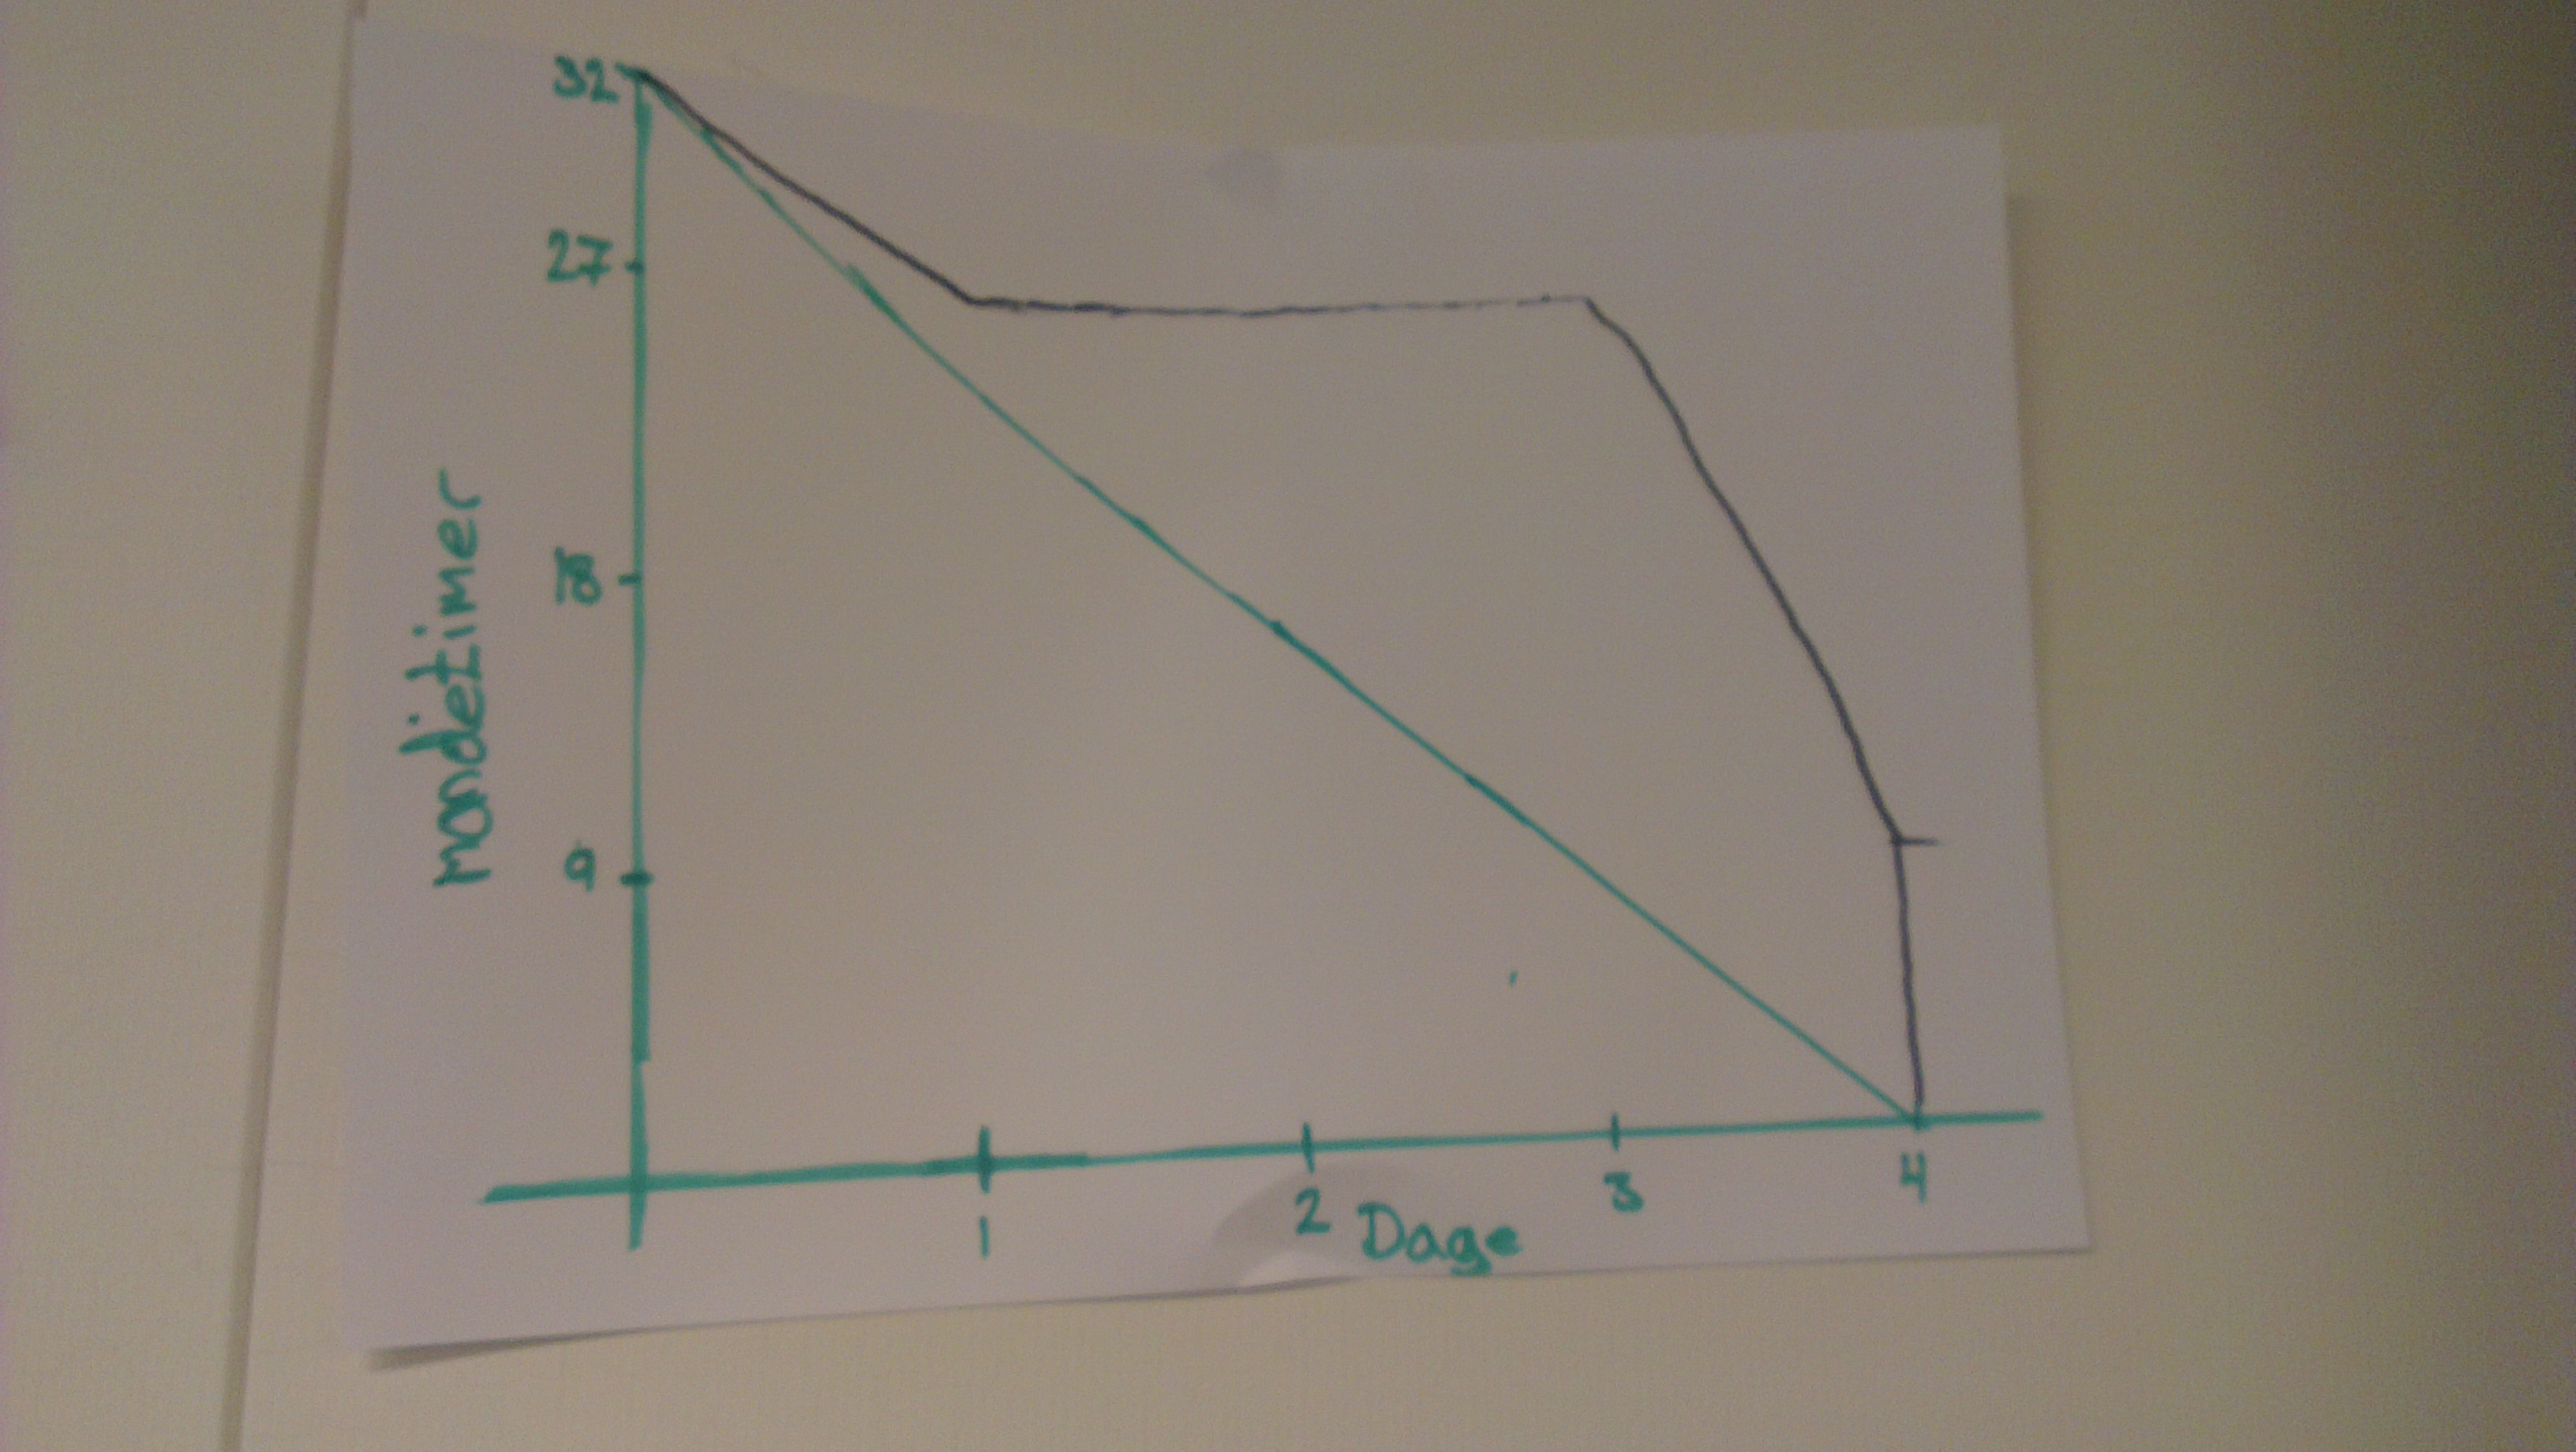
\includegraphics[scale=0.10]{includes/billeder/sprint2.jpg}
\subsubsection*{Product backlog}
Backlog lavet den 9.12.2013 i starten af sprint 2. \\
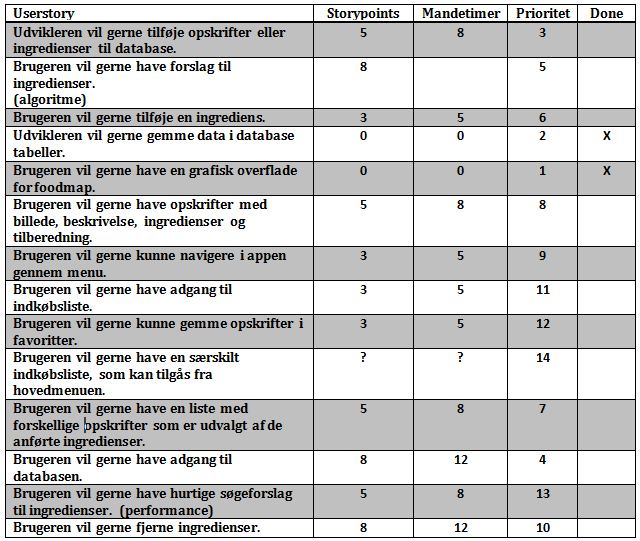
\includegraphics[scale=0.60]{includes/billeder/productbacklog_sprint2.png}

\subsubsection*{Sprint backlog}
I sprint 2 fokuserede vi p� f�lgende userstories: \\
Database kobling, dummy data til databasen, algoritme. \\
Samt database tabeller og basic gui som vi satte til 0 mandetimer eftersom delene var f�rdige efter at have opdelt dem, da de var for store. 

\subsection*{Xp og scrum praktikker}
I sprint 2 benyttede vi XP praktikkerne: stand-up meeting, planning poker, par programmering, kollektivt kode ejerskab, refactoring, kodestandarder, metafor og simpelt design. \\
Vi havde en scrum master, men product owner droppede vi lidt da det ikke giver s� meget mening i en gruppe af 3. \\
Vi lavede planning poker med storypoints til at vurdere st�rrelsen af userstories for senere hen at udregne vores velocity. \\

\subsection*{Forl�b}

\subsection*{Produkt review}
Til produkt reviewet var det planen at vi ville vise vores gui med database adgang, men emuleratoren fejlede og pr�sentationen faldt til bunden. Derfor endte det med at vi kun kunne vise selve databasen med data. 

\subsubsection*{Konklusion af review}
Vi skulle have v�ret lidt bedre forberedt til reviewet, dermed det m�ske v�ret muligt at undg� problemer med emulatoren og kunden havde f�et et bedre indtryk.

\subsection*{Retrospektive}
I sprintet blev vi f�rdige med databaseadgangen. \\
Vi havde overvurderet hvor mange resurser vi havde til r�dighed.

\subsubsection*{Hvad gik godt}

\subsubsection*{Hvad gik mindre godt}

\subsubsection*{Hvad �ndrer vi til n�ste sprint}

\newpage